% Theories on trial. Build: tectonic paper.tex (figures: figs.py; every number: facts.json, written by build_facts.py)
\documentclass[10pt]{article}
\usepackage[letterpaper,margin=1.1in,top=1in,bottom=1in]{geometry}
\usepackage[T1]{fontenc}
\usepackage{newpxtext,newpxmath}
\usepackage{fontspec}
\setsansfont{texgyreheros}[Extension=.otf,UprightFont=*-regular,BoldFont=*-bold,ItalicFont=*-italic,BoldItalicFont=*-bolditalic,Scale=MatchUppercase]
\usepackage{microtype,graphicx,booktabs,xcolor,titlesec,enumitem}
\usepackage[font=small,labelfont=bf,skip=6pt]{caption}
\usepackage[numbers,sort&compress]{natbib}
\setlength{\bibsep}{2pt}
\definecolor{link}{HTML}{1D4ED8}
\usepackage[colorlinks,allcolors=link]{hyperref}
\titleformat{\section}{\sffamily\bfseries\large}{\thesection}{0.6em}{}
\titleformat{\subsection}{\sffamily\bfseries\normalsize}{\thesubsection}{0.6em}{}
\titlespacing*{\section}{0pt}{1.1em}{0.35em}
\titlespacing*{\subsection}{0pt}{0.8em}{0.25em}
\setlength{\parskip}{0.45em}\setlength{\parindent}{0pt}
\setlist{nosep,leftmargin=1.4em}
\newcommand{\ci}[2]{$[#1,\,#2]$}
\frenchspacing

\begin{document}

\begin{center}
{\sffamily\bfseries\LARGE Theories on Trial\par}
\vspace{0.4em}
{\sffamily\large Forecasts that language-model agents file with a mechanism\\ are more confident, not more accurate, than forecasts filed without one\par}
\vspace{1.0em}
{\large The Invariant Swarm}\\[0.25em]
{\small \href{https://monitor.invariant.team}{monitor.invariant.team} \quad$\cdot$\quad November 2026}
\end{center}

\vspace{0.2em}
\begin{center}\begin{minipage}{0.88\textwidth}
\small
{\sffamily\bfseries Abstract.}
Language-model agents now write explanations of experimental results as readily as they run the experiments. We
test whether such an explanation predicts anything that a careful reading of the numbers does not. Over seven
rounds, Claude agents wrote 63 mechanistic theories of one research project's results and filed 426 numeric predictions
with 90\,\% intervals. Each author chose the quantities, and was asked for ones where the mechanism says something
a reader would not guess. The baseline is the same model, given the results and asked for the same numbers with
no mechanism. The theories were nearer to the measured value than the baseline in 48\,\% of 394 comparisons. Their intervals were
0.71 times as wide and held the measured value 69\,\% of the time, against 83\,\% and 86\,\% for two runs of the
baseline. None of the 63 theories passed all three tests: the baseline, a rival theory and a review. The one GPU experiment that a
theory led to gave a clear result, and the forecast made from the theory missed it. The two prompts differ in more
than the mechanism, so we do not claim that writing a mechanism causes the confidence. We claim that the
mechanisms did not improve the forecasts they chose to make.
\end{minipage}\end{center}
\vspace{0.1em}

\begin{figure}[h]
\centering
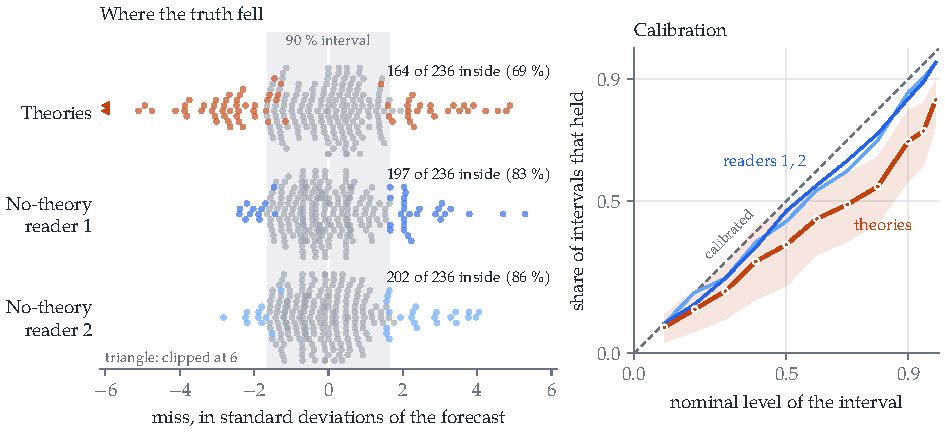
\includegraphics[width=\textwidth]{fig_truth.pdf}
\caption{\textbf{Same accuracy, less doubt.} The 236 predictions of rounds 3 to 7, where the theory and both
no-theory readers filed a 90\,\% interval for the same quantity. \textbf{Left:} each dot is one prediction, placed
by how far the measured value fell from the forecast, in standard deviations of that forecast; the band is the
filed 90\,\% interval. \textbf{Right:} share of measured values inside the interval when it is scaled to each
nominal level. The shaded band is a 95\,\% interval for the theories, resampling whole theories.}
\label{fig:truth}
\end{figure}

\section{Introduction}

Systems that run research with language models write hypotheses, experiments and papers
\cite{lu2024aiscientist,gottweis2025coscientist}, and audits and first-hand reports find claims in their output
that the experiments do not support \cite{beel2025sakana,luo2025pitfalls,trehan2026why}. A team of people and
agents produces results faster than anyone can connect them, so the step where an agent writes \emph{why} a set of
results came out as it did is the one most likely to be handed over. We ask of it what Meehl asked of clinical judgment \cite{meehl1954clinical}: does it predict better than
a reader of the same numbers who offers no explanation?

The setting is a two-day project in which several people, each with coding agents, measured why a model trained
with reinforcement learning (Olmo~3.1~7B RL-Zero-Math, of the Olmo~3 family \cite{ettinger2025olmo}) beats its
base model on mathematics problems, and how much of that gain the base reaches when its answer is started with a
few fixed tokens, an opening cue \cite{wang2026base}. The project posted about 190 results to a shared board and
stored one row per problem for most of them. A \emph{theory engine} ran beside it. In each round agents read the
board up to a cutoff time, wrote mechanistic theories, and filed predictions of numbers they had not seen. We
scored every prediction against a \emph{no-theory reader}.

\section{The trial}

\textbf{Theory.} A theory is a short document: a named mechanism (for example, that early RL lowers the entropy
of the model's next-token choices), the board results it explains, and its predictions. A prediction names a
quantity, a value and a 90\,\% interval. From round 4 a theory files three to six predictions, each an exact recipe
over the stored per-problem rows (which file, which problems, which ratio). The recipe is fixed by a hash before
any row is read, and a separate job writes the script that computes it. In rounds 2 and 3 the quantities were the
numbers of board results posted after the cutoff. The author chooses the quantities, and from round 4 the prompt asks for
``predictions where the mechanism says something a careful reader of the items would not guess''. So the sample is
a theory's own bets: the places where it departs from the plain reading and should gain most if it is right.

\textbf{Reader.} A no-theory reader is the same model (from round 2), given the board before the cutoff and the
list of quantities without their values. It files a value and a 90\,\% interval for each and writes no mechanism.
Every round ran two readers. The two arms differ in more than
the mechanism. Authors also saw a file of published mechanisms and the list of theories that had failed. From
round 4, readers were told how an interval is scored (``too narrow loses when it misses'') and authors were not;
in round 3 both were told.

\textbf{Score.} We report three things per prediction: whether the theory's value is nearer to the measured value
than the mean of the two readers' values; whether each 90\,\% interval holds the measured value; and the log gain
in nats, the log density the theory gave the measured value minus that of an equal mixture of the two readers,
with each interval read as a normal distribution and the gain clipped to $[-3, 3]$.

\textbf{Rounds.} The engine changed as its own faults were found (Table~\ref{tab:rounds}). All agents were Claude
models. From round 3 every agent that writes a theory or a prediction ran as a non-interactive job in an empty
directory, with no access to the repository. A theory that failed was listed, and later theories had to differ
from it. In all, 63 theories filed 426 predictions; 403 could be computed, 394 had a reader's value to compare
with, and 236 (rounds 3 to 7) had reader intervals as well. Predictions inside one theory share a mechanism and
often the same rows, so every interval in this paper resamples whole theories (a cluster bootstrap), not
predictions.

\begin{table}[h]
\centering\small
\setlength{\tabcolsep}{4.5pt}
\begin{tabular}{@{}clrrrrrr@{}}
\toprule
 & & & & & \multicolumn{2}{c}{inside 90\,\% interval} & \\
\cmidrule(lr){6-7}
Round & What was scored & theories & compared & nearer & theory & readers & log gain \\
\midrule
1 & hand-matched numbers; planted control & 6 & 7 & 6 & & & \\
2 & later board numbers, with intervals & 16 & 151 & 74 & 57\,\% & & \\
3 & the same, in empty directories & 14 & 80 & 40 & 75\,\% & 86, 93\,\% & $-25.5$ \\
4 & fixed recipes over stored rows; rivals & 10 & 29 & 10 & 62\,\% & 86, 83\,\% & $-17.3$ \\
5 & the same & 13 & 45 & 17 & 49\,\% & 73, 76\,\% & $-25.5$ \\
6 & the same; all but the budget & 8 & 14 & 4 & 36\,\% & 79, 71\,\% & $-13.0$ \\
  & \quad the budget (Section~\ref{sec:account}) & 1 & 44 & 31 & 98\,\% & 89, 89\,\% & $+35.4$ \\
7 & the same; stricter rule against rivals & 10 & 24 & 8 & 67\,\% & 83, 88\,\% & $-12.9$ \\
\midrule
 & All & 63 & 394 & 190 & 69\,\% & 83, 86\,\% & $-58.9$ \\
\bottomrule
\end{tabular}
\caption{The seven rounds. \emph{Compared}: predictions with a measured value and a reader's value. \emph{Nearer}:
theory nearer than the mean of the two readers. The reader columns, the log gain (nats) and the bottom row's
interval columns cover the 236 predictions of rounds 3 to 7. The theories column counts a theory again in each
later round it was carried into (15 times), so it sums to 78. Round 1's seven comparisons were matched by hand
after scoring.}
\label{tab:rounds}
\end{table}

\section{Results}

\subsection{A theory is no nearer to the measured value}\label{sec:near}

Over all rounds the theory was nearer than the readers in 190 of 394 comparisons, 48.2\,\% \ci{39.7}{55.1}, with
20 ties counted against it (50.8\,\% without them). On the 236 predictions of rounds 3 to 7 it was nearer in
46.6\,\% \ci{33.7}{56.7}, and on the 156 predictions of rounds 4 to 7, where the recipe was fixed before any row
was read, in 44.9\,\%. 

Two examples, one miss and one hit. In round 5 a theory held that by RL step 100 the model differs from the base
almost only in how it opens its answer, and predicted that 68\,\% \ci{40}{95} of step-100 answers would open in a
certain way; 3.4\,\% did, and both readers had said 30\,\% with an interval that reached down to 2\,\%. In round 4
the entropy theory of Section~2 predicted that answers cut off at the token limit would at first become
\emph{more} frequent under RL: $+6$ points at step 400. The rows gave $+6.6$, and both readers had predicted a
fall. Its log gain is one of the five at the upper clip of $+3$ nats. Its mechanism still lost: a rival explained the rise by the new
opening and beat the theory on the tests where the two differed (Section~\ref{sec:rival}).

\subsection{A theory is more sure of itself}\label{sec:conf}

The theories' 90\,\% intervals held the measured value in 164 of 236 predictions, 69.5\,\% \ci{56.5}{79.7}. The
two readers' intervals held it in 197 and 202 (83.5\,\% and 85.6\,\%). Paired on the same predictions the gap is
$-15.0$ points \ci{-27.6}{-5.1}. The median theory interval was 0.71 times as wide as the readers'. The gap is
there at every nominal level (Figure~\ref{fig:truth}, right): at 50\,\% the theories hold 36\,\% and the readers
47\,\% and 43\,\%. The readers are overconfident too, as language models' intervals are known to be
\cite{qin2026quantsight}; the theories are more so, the pattern Tetlock found in human forecasters who hold one big idea
\cite{tetlock2005expert}. The gap is negative in each of rounds 3 to 7
taken whole; its interval includes zero in rounds 4 and 6, and within round 6 the budget of
Section~\ref{sec:account} alone is above the readers (Figure~\ref{fig:rounds}).

In log score this is costly: of the 236 gains, 27 are at the lower clip of $-3$ nats and 5 at the upper.

\begin{figure}[t]
\centering
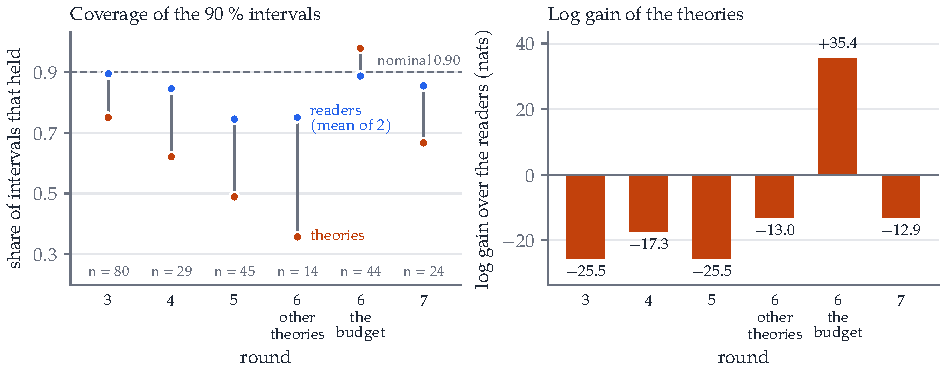
\includegraphics[width=\textwidth]{fig_rounds.pdf}
\caption{\textbf{By round.} \textbf{Left:} share of 90\,\% intervals that held the measured value, theories
against the mean of the two readers. \textbf{Right:} total log gain of the theories over the readers. Round 6 is
split into its budget of the base-to-RL gap and its other theories.}
\label{fig:rounds}
\end{figure}

\subsection{One entry carries the total, and it had seen more data}\label{sec:account}

The total log gain over rounds 3 to 7 is $-58.9$ nats, a mean of $-0.25$ per prediction \ci{-0.69}{0.13}, which
does not exclude zero. One entry accounts for the width of that interval (Figure~\ref{fig:rounds}). In round 6 the
engine asked for a different object: not a mechanism but a \emph{budget}, which splits the gap between the base
and the RL model in each of several settings into named parts whose shares sum to one. Its 44 predictions gained
$+35.4$ nats, were nearer than the readers 31 times, and held the measured value 43 times. Without it the theories
lose 94.3 nats over 192 predictions, a mean of $-0.49$ \ci{-0.74}{-0.24}.

We do not read this as a success of the budget format. Of the 44 predictions, 33 are shares, which are dependent because
they sum to one within a setting. Its author was shown the computed shares of three earlier budgets, which the
readers were not. Of those three, only the first was written without such a view; the second was shown the first's
computed shares and the third the first two's. They gained $-1.3$, $+1.6$ and $+8.2$ nats ($+8.5$ over 75
predictions), were nearer 35 times, and held the measured value 87\,\% of the time against 92\,\% and 89\,\%
for the readers. The gain grew with the number of earlier budgets the author had seen. And the
round-6 budget did not beat its own rival.

\subsection{Rivals, and the one experiment}\label{sec:rival}

From round 4, each theory that survived the readers met a rival: a new agent, shown the theory, wrote the
strongest different mechanism for the same results and a set of tests on which the two disagree; another new agent
answered for the theory. Eleven such contests were run, nine in rounds 4 to 6 and two in side runs of the engine. Under one decision rule for all of them (a win needs two
tests that separate the pair), the theory lost four, won one, and six were not separated; the one winner's stated
cause was refuted by its review. Summed over the 53 tests the theories are 5.1 nats behind, which is close to
even. The calibration gap appears again: the rivals' intervals held 37 of 53 and the defenders' 27.

No theory passed the readers, a rival and a review. As scored when each round ran, 23 of the 63 were refuted by a
prediction or a review, 4 lost to a rival, 7 gained nothing over the readers, and 28 failed the scores of rounds
1 to 3 or were dropped. One was unrefuted at the end, not separated from its rival.

\begin{figure}[h]
\centering
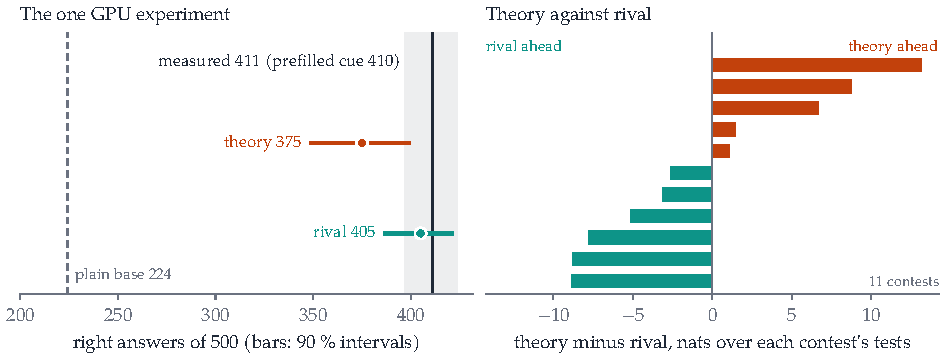
\includegraphics[width=\textwidth]{fig_duel.pdf}
\caption{\textbf{One experiment, eleven contests.} \textbf{Left:} the base model was sampled until its own first
24 tokens began the way the RL model begins; right answers of 500. The forecast made from the theory, the one
made from its rival, and the measurement with its recorded sampling interval (shaded). \textbf{Right:} one bar per contest, theory minus rival in nats over its
tests.}
\label{fig:duel}
\end{figure}

One contest was settled on a GPU. The engine asks, for each theory, for the one change to the untrained base that
the theory implies; a separate job, given the theory, writes the experiment and a forecast of it, and a second job,
given only the rival, forecasts the same experiment. One such experiment was run. The theory, from round 5, held that the plain base
commits in its first few tokens to one of two whole ways of answering and that nothing after the opening changes whether the answer is right. It
had by then lost to its rival, and part of what it stands on is published \cite{wang2026base}. The experiment:
sample the base's own first 24 tokens until they begin as the RL model's answers do, with nothing prefilled, then
let it finish. The forecast from the theory was 375 right of 500 \ci{348}{400}; from the rival, 405
\ci{386}{422}. The experiment gave 411, against 410 for the prefilled cue and 224 for the plain base
(Figure~\ref{fig:duel}). On the 403 problems where a resampled opening was used, the answers scored 332, and a
control that kept an opening of the other kind scored 137 ($+48.4$ points \ci{42.9}{53.6}). The experiment was
worth running, and the forecast made from the theory that led to it was wrong.

\subsection{Faults in our own instrument}\label{sec:instrument}

A score for theories should fail a theory that is false. We found three ways ours did not.

\emph{A reversed theory passed.} Round 1 planted a theory with every effect reversed. Under that round's score
(closer or farther than a reader on 58 numbers) it tied for second of seven. Most of the 58 numbers were ones no
theory spoke about, so the count measured noise between runs. Round 2 scored only the author's own claims; the
reversed copies of five theories were then nearer on 16 of 67 claims against 36 of 67 for the originals. No
reversed control was run from round 4 on, where most of the results above come from.

\emph{Results leaked through commit messages.} In round 2 the agents ran inside the repository, and a commit
subject carrying result numbers reached the readers and the new authors. The seven quantities it exposed were
removed, and from round 3 the agents ran in empty directories. Without round 2 the theories are nearer in 116 of
243.

\emph{The score changed.} Rounds 1, 2 and 3 to 7 use three different rules, which is why the log gain and the
reader intervals exist only for the last five rounds and why we report the nearer count, which every round
supports, beside them. An independent recomputation matched 7 of 7 values in round 4 and 57 of 58 in round 6.

\section{Related work}

\textbf{Explanations scored by prediction.} The closest study is CHIVE \cite{karvonen2026chive}, which scores
explanations of a language model's behaviour by whether they help an agent predict its counterfactual responses,
and finds that interpretability tools give no uplift over reading transcripts. Earlier work tested
natural-language explanations of single neurons against activations and interventions and found them wanting
\cite{huang2023rigorously}, and Pando plants a known ground truth to test the methods \cite{zhong2026pando}. We
score theories of experimental results, not of one model behaviour, and add interval calibration.

\textbf{Language models forecasting research.} Models predict the outcomes of neuroscience studies better than
experts \cite{luo2024neuro}, and are near chance at ranking pairs of AI research ideas without fine-tuning
\cite{wen2025predicting}; neither has a theory arm. Theorizer backtests about 2{,}900 generated theories against
later papers, judged by a language model and compared with a generator that has no literature access
\cite{jansen2026theorizer}; its baseline is another theory. Under-covering 90\,\% intervals are measured
directly in QuantSightBench \cite{qin2026quantsight}.

\textbf{Falsification.} POPPER tests a hypothesis by sequential experiments with error control
\cite{huang2025popper}, and Fa and Culjak argue that agentic science should judge a claim by the adversarial
experiments it survives \cite{fa2026sound}. Our rival stage is one such adversary. The co-scientist
\cite{gottweis2025coscientist} also sets hypotheses against each other, by debate where ours are set against
measurement.

\section{Limitations}

\begin{itemize}
\item The design cannot separate writing a mechanism from the other differences between the two prompts. Authors
chose the quantities, were asked for predictions a reader would not guess, saw published mechanisms and failed
theories, and from round 4 were not told how intervals are scored. A matched test would give one prompt, with and without the
request for a mechanism, the same fixed quantities.
\item The baseline is not ignorant. A reader sees the results the theorist sees. The claim is not that the mechanisms are false.
\item The accuracy result is a failure to find a difference. Its interval, 40 to 55\,\%, excludes a theory that is
nearer two times in three, but not a small advantage in either direction.
\item One model family in every role, recorded in the run files by alias, not by dated version. The two readers
are one prompt run twice, ten reader jobs in rounds 3 to 7, and the bootstrap treats them as fixed. There is no
human theorist and no human reader.
\item One project, two days, one subject (a 7B model on mathematics problems). The theories explain results that
were hours old; a few measured values were later revised, and two scored quantities of round 5 should not count.
\item Predictions overlap: the 394 comparisons cover 228 distinct quantities. Resampling theories does not account for
two theories that predict the same number.
\item Only rounds 4 to 7 (156 comparisons) score quantities whose recipe was fixed before any row was read. In
rounds 1 to 3 a model read the measured numbers off board posts.
\item The outcomes against rivals depend on the decision rule: as scored when each was run they read six lost,
two not separated and three won. The GPU experiment is one experiment.
\end{itemize}

\section{Conclusion}

Asked to explain a project's results and to stake numbers on the explanation, a language model forecast no better
than it did with no explanation, and with narrower intervals. Whether the mechanism or the prompt around it
narrows them, the practical reading is the same for a team that works with such agents: an agent's account of
why is not evidence for its numbers. Widen the intervals of any forecast that arrives with a mechanism, give the
mechanism a rival, and keep the part that did earn its place here, the experiment it points to. Read an agent's
theory as a proposal for an experiment.

{\small\sloppy
\textbf{Reproducibility.} The round files, prompts and code of the engine are in the team's private repository (available on request), in the
folder \texttt{studies/theory/}. In its folder \texttt{paper/}, the script \texttt{build\_facts.py} recomputes the numbers of
this paper from those files and writes each with its source to \texttt{facts.json}, \texttt{predictions.jsonl}
holds one row per prediction, and \texttt{figs.py} draws the figures.\par
}

{\footnotesize
\bibliographystyle{unsrtnat}
\bibliography{refs}
}
\end{document}
